\documentclass[11pt,a4paper]{article}
\usepackage[margin=1in]{geometry}
\usepackage[utf8]{inputenc}
\usepackage{amsmath}
\usepackage{xcolor}
\usepackage[english]{babel}
\usepackage{amsthm}
\usepackage{amsfonts}
\usepackage{mathrsfs}
\usepackage{mathtools}
\usepackage{algorithm}
\usepackage{algpseudocode}
\usepackage{amssymb}
\usepackage{enumerate}
\usepackage[hidelinks]{hyperref}
\usepackage{cancel}

\hypersetup{
    colorlinks=true,
    linkcolor=blue,
    filecolor=magenta, 
    citecolor=magenta,     
    urlcolor=blue,
    pdftitle={Information Theory},
    pdfpagemode=FullScreen,
}


\author{Jayadev Naram}
\title{Information Theory} 

\begin{document}

\date{}
\maketitle
\tableofcontents
% \newpage

\theoremstyle{plain}
\newtheorem{theorem}{Theorem}[section]
\newtheorem{corollary}[theorem]{Corollary}
\newtheorem{lemma}[theorem]{Lemma}
\newtheorem{proposition}[theorem]{Proposition}
\newtheorem{assume}{Assumption}

\theoremstyle{definition}
\newtheorem{definition}[theorem]{Definition}
\newtheorem{example}[theorem]{Example}
\newtheorem*{problem*}{Problem}
\newtheorem{remark}[theorem]{Remark}

\newcommand{\red}[1]{{\color{red}#1}}

\newcommand{\independent}{\perp\!\!\!\!\perp} 
\newcommand{\divergence}[2]{\mathscr{D} \left(#1\|#2\right)} 
\newcommand{\supp}[1]{\text{supp}\left( #1 \right)}
\newcommand{\YgX}{{Y|X}}
\newcommand{\XY}{{X,Y}}
\newcommand{\Var}{\mathbb{V}\text{ar}}

\newcommand{\R}{\mathbb{R}}
\newcommand{\A}{\mathcal{A}}
\newcommand{\M}{\mathcal{M}}
\newcommand{\U}{\mathcal{U}}
\newcommand{\X}{\mathcal{X}}
\newcommand{\C}{\mathcal{C}}
\newcommand{\T}{\mathcal{T}}
\newcommand{\Y}{\mathcal{Y}}
\newcommand{\E}{\mathbb{E}}
\newcommand{\barl}{\bar{\ell}}
\newcommand{\barL}{\bar{L}}
\newcommand{\N}{\mathcal{N}}
\newcommand{\h}{\mathcal{H}}
\newcommand{\Prob}{\mathbb{P}}
\newcommand{\Dist}{\mathcal{D}}
\newcommand{\perpProj}{\mathcal{P}^\perp}
\newcommand{\bb}{\mathbb{B}}
\newcommand{\Sprod}{\mathbb{S}_{xy}}
\newcommand{\highlight}[1]{\textit{\textbf{#1}}}
\newcommand{\mapping}[3]{#1:#2\rightarrow #3}
\newcommand{\doubt}{\highlight{[??]}}
% \newcommand{\bigvert}[2]{#1{\raisebox{-.5ex}{$|$}_{#2}}}
\newcommand{\bigvert}[2]{\left.#1\right|_{#2}}
\newcommand{\sdnn}[1]{${#1}$}
\newcommand{\bsdnn}[1]{$\boldsymbol{#1}$}
\newcommand{\ifthen}[2]{\textbf{(#1)}\boldsymbol{\implies}\textbf{(#2)}}
\newcommand{\bsdn}[1]{\boldsymbol{#1}}
\newcommand{\forward}{$(\implies)$}
\newcommand{\converse}{$(\impliedby)$}
\newcommand{\Lt}[1]{\underset{#1\rightarrow 0}{Lt}}
\newcommand{\norm}[1]{\|#1\|}
\newcommand{\dparder}[2]{\dfrac{\partial #1}{\partial x_{#2}}}
\newcommand{\fparder}[2]{\frac{\partial #1}{\partial x_{#2}}}
\newcommand{\parder}[2]{\partial #1/\partial x_{#2}}
\newcommand{\parop}[1]{\dfrac{\partial}{\partial x_{#1}}}
\newcommand{\innerproduct}[2]{\langle #1, #2 \rangle}
\newcommand{\genst}{St_B(n,p)}
\newcommand{\igenst}[1]{St_{B_{#1}}(n_{#1},p)}
\newcommand{\realmat}[2]{\R^{#1\times #2}}
\newcommand{\Skew}{\mathcal{S}_{skew}(p)}
\newcommand{\Sym}{\mathcal{S}_{sym}(p)}
\newcommand{\XperpB}{X_{B^\perp}}
\newcommand{\polarRetr}{R^{polar}_X}
\newcommand{\qrRetr}{R^{QR}_X}
\newcommand{\vectransport}{\mathcal{T}}
\newcommand{\grad}{\text{grad}\,}
\newcommand{\hess}{\text{Hess}\,}

\nocite{*}

\section{Entropy}

\begin{definition}
    The \highlight{uncertainity or entropy} of a discrete random variable $U$ that takes values in the set $\mathcal{U}$ (also called alphabet $\mathcal{U}$) is defined as 
    \begin{equation*}
        H(U) = -\sum_{u\in \mathcal{U}} P_U(u) \log_b P_U(u),
        % H(U) = -\sum_{u\in \text{supp}(P_U)} P_U(u) \log_b P_U(u),
    \end{equation*}
    where $P_U(\cdot)$ denotes the probability mass function of the random variable $U$.
    % , and the 
\end{definition}

\begin{remark}
    It should be noted that when $P_U(u) = 0$, the corresponding term does not contribute to entropy because $\lim_{t\downarrow 0} t\log_b t = 0$. In view of this result, one can equivalently define entropy on the support of $P_U$ which is defined as
    \begin{equation*}
        \text{supp}(P_U) = \{u\;:\; P_U(u)>0 \} \subseteq \mathcal{U}.
    \end{equation*}
\end{remark}

\begin{remark}
    Entropy does not depend on different possible values that $U$ can take on, but only on the probabilities of these values.
\end{remark}

\begin{definition}
    If $U$ is binary with two possible values $u_1$ and $u_2$, such that $\Prob[U = u_1] = p$ and $\Prob[U = u_2] = 1-p$, then 
    \begin{equation*}
        H(U) = H_b(p) = -p\log_2 p -(1-p)\log_2 (1-p), p\in[0,1],
    \end{equation*}
    where $H_b(\cdot)$ is called the \highlight{binary entropy function}.
\end{definition}

\begin{definition}
    Let $f$ be a function from a convex set $C$ to $\R$. Then $f$ is said to be \highlight{convex function} on $C$ if for every $x,y\in C$ and $0\le\lambda \le 1$,
    \begin{equation*}
        f((1-\lambda)x+\lambda y) \le (1-\lambda) f(x) + \lambda f(y).
    \end{equation*} 
    A function is said to be \highlight{strictly convex} if equality holds only if $\lambda = 0$ or $\lambda = 1$. A function $f$ is \highlight{concave} if $-f$ is convex.
\end{definition}

\begin{lemma}
    Let $\mapping{f}{\R}{\R}$ be a twice continuously differentiable function on an open set $E$. Then $f$ is convex on $E$ iff its second derivative $f^{\prime\prime}$ is nonnegative throughout $E$. If $f^{\prime\prime}$ is positive on $E$, then $f$ is strictly convex.
\end{lemma}

\begin{remark}
    Notice that $-\log x$ and $x\log x$ are strictly convex on $(0,\infty)$.
\end{remark}

\begin{lemma}[\highlight{Jensen's Inequality}]
    Let $\mapping{f}{\R}{\R}$ be a convex function. Then 
    \begin{equation*}
        f\Big(\sum_{i=1}^n\lambda_i x_i\Big)\le \sum_{i=1}^n\lambda_i f(x_i),
    \end{equation*}
    where $\lambda_i\ge 0\ \forall\ i$, $\sum_{i=1}^n\lambda_i = 1$ and equality holds iff $x_1 = \cdots = x_n$ or $f$ is linear.
\end{lemma}

\begin{remark}
    If $f$ is strictly convex which rules out the linearity, the equality of Jensen inequality holds iff $x_1 = \cdots = x_n$.
\end{remark}

\begin{remark}
    Suppose $X$ is a discrete random variable over an alphabet $\mathcal{X} = \{x_1,\ldots,x_n\}$ and $f$ is a strictly convex function on $\R$. Then by setting $\lambda_i = P_X(x_i)$, we have 
    \begin{equation*}
        f(\E[X])\le \E[f(X)],
    \end{equation*}
    where equality holds iff $x_1 = \cdots = x_n$, i.e., $X$ is a constant.
\end{remark}

% \begin{lemma}[IT Inequality]
%     For any base $b>1$ and any $\xi > 0$, 
%     \begin{equation*}
%         \bigg(1-\dfrac{1}{\xi}\bigg)\log_b e \le \log_b \xi \le (\xi-1) \log_b e,
%     \end{equation*}
%     with equalities on both sides hold iff $\xi = 1$.
% \end{lemma}

\begin{theorem}
    If $U$ has $r$ possible values, then 
    \begin{equation*}
        0 \le H(U)\le \log r,
    \end{equation*}
    where 
    \begin{align*}
        H(U) = 0\quad &\iff \exists\ u\in\mathcal{U}, P_U(u) = 1, \\
        H(U) = \log r &\iff \forall\ u\in\mathcal{U}, P_U(u) = \dfrac{1}{r}.
    \end{align*}
\end{theorem}

\begin{proof}
    Since $0\le P_U(u) \le 1$, we have 
    \begin{equation*}
        -P_U(u)\log_2 P_U(u) \begin{cases}
            = 0\quad \text{if } P_U(u) = 1,\\
            > 0\quad \text{if } 0 < P_U(u) < 1.
        \end{cases}
    \end{equation*}
    Hence, $H(U) \ge 0$. Equality can only be achieved if $-P_U(u)\log_2 P_U(u) = 0$ for all $u\in \text{supp}(P_U)$, i.e., $P_U(u) = 1$ for all $u\in \text{supp}(P_U)$.

    To derive the upper bound we use a trick that is quite common in information theory: We take the difference and try to show that it must be nonpositive:
    \begin{align*}
        H(U) - \log r &= - \sum_{u\in\U} P_U(u)\log P_U(u) - \log r \\
        &= \sum_{u\in\U} P_U(u)\log \dfrac{1}{P_U(u) r} \\
        &\le \log\bigg( \sum_{u\in\U} P_U(u) \dfrac{1}{P_U(u) r} \bigg) = 0,
    \end{align*}
    where we have used the strict concavity of $\log x$ and Jensen inequality. Equality holds iff $\dfrac{1}{P_U(u) r} = 1$ for all $u\in \U$, i.e., $P_U(u) = \dfrac{1}{r}$ for all $u\in U$.
\end{proof}

\begin{definition}
    The \highlight{conditional entropy} of the random variable $X$ given the event $Y = y$ is defined as 
    \begin{equation*}
        H(X|Y = y) = -\sum_{x\in \mathcal{X}} P_{X|Y}(x|y) \log P_{X|Y}(x|y) = -\E\Big[\log P_{X|Y}(X|Y)\Big| Y = y \Big],
    \end{equation*}
    where the conditional probability distribution is given by
    \begin{equation*}
        P_{X|Y}(x|y) = \dfrac{P_{X,Y}(x,y)}{P_Y(y)}.
    \end{equation*}
\end{definition}

\begin{corollary}
    If $X$ has $r$ possible values, then 
    \begin{equation*}
        0 \le H(X|Y = y)\le \log r,
    \end{equation*}
    where 
    \begin{align*}
        H(X|Y = y) = 0\quad &\iff \exists\ x\in\mathcal{X}, P_{X|Y}(x|y) = 1, \\
        H(X|Y = y) = \log r &\iff \forall\ x\in\mathcal{X}, P_{X|Y}(x|y) = \dfrac{1}{r}.
    \end{align*}
\end{corollary}

\begin{definition}
    The \highlight{conditional entropy} of the random variable $X$ given the random variable $Y$ is defined as 
    \begin{align*}
        H(X|Y) &= \sum_{y\in \mathcal{Y}} P_{Y}(y) H(X|Y = y)\\
        &= \E_Y\big[H(X|Y = y)\big] \\
        &= -\sum_{x\in \mathcal{X},y\in \mathcal{Y}} P_{X,Y}(x,y) \log P_{X|Y}(x|y)\\
        &= -\E\Big[\log P_{X|Y}(X|Y) \Big].
    \end{align*}
\end{definition}

\begin{corollary}
    If $X$ has $r$ possible values, then 
    \begin{equation*}
        0 \le H(X|Y)\le \log r,
    \end{equation*}
    where 
    \begin{align*}
        H(X|Y) = 0\quad &\iff \exists\ x\in\mathcal{X}, \forall\ y\in \mathcal{Y}, P_{X|Y}(x|y) = 1, \\
        H(X|Y) = \log r &\iff \forall\ x\in\mathcal{X}, \forall\ y\in \mathcal{Y}, P_{X|Y}(x|y) = \dfrac{1}{r}.
    \end{align*}
\end{corollary}

\begin{remark}
    Generally, $H(X|Y)\neq H(Y|X)$.
\end{remark}

\begin{theorem}[\highlight{Conditioning Reduced Uncertainity}]\label{thm:conditioning_reduces_entropy}
    For any two discrete random variables $X$ and $Y$,
    \begin{equation*}
        H(X|Y)\le H(X),
    \end{equation*}
    where equality holds iff $X$ and $Y$ are independent, i.e., $X \independent Y$.
\end{theorem}

\begin{proof}
    Consider the following:
    \begin{align*}
        H(X|Y) - H(X) &= -\sum_{x\in \X, y\in \Y} P_{X,Y}(x,y) \log P_{X|Y}(x|y) + \sum_{x\in \X, y\in \Y} P_{X,Y}(x,y) \log P_{X}(x) \\
        &= \sum_{x\in \X, y\in \Y} P_{X,Y}(x,y) \log \dfrac{P_{X}(x)}{P_{X|Y}(x|y)} \\
        &= \sum_{x\in \X, y\in \Y} P_{X,Y}(x,y) \log \dfrac{P_{X}(x)P_{Y}(y)}{P_{X,Y}(x,y)} \\
        &\le \log \bigg( \sum_{x\in \X, y\in \Y} P_{X,Y}(x,y) \dfrac{P_{X}(x)P_{Y}(y)}{P_{X,Y}(x,y)}\bigg) \\
        &= \log \bigg(\Big(\sum_{x\in \X} P_{X}(x)\Big) \Big(\sum_{y\in \Y}P_{Y}(y)\Big)\bigg) = 0,
    \end{align*}
    where we have used the strict concavity of $\log x$ and Jensen inequality. Equality holds iff $\dfrac{P_{X}(x)P_{Y}(y)}{P_{X,Y}(x,y)} = 1$ for all $x\in \X$ and $y\in \Y$, i.e., $X\independent Y$.
\end{proof}

\begin{remark}
    The conditioning reduces entropy-rule only applies to random variables, but not to events. In particular,
    \begin{equation*}
        H(X|Y = y) \lesseqgtr H(X).
    \end{equation*}
    To understand why this is the case, consider the following example. Suppose $X,Y$ are random variables such that $P_X(x_1) = 0.4, P_X(x_2) = 0.6$, $P_{X|Y}(x_1|y_1) = 1$ and $P_{X|Y}(x_i|y_2) = 1/2, i = 1, 2$. Then we see that 
    \begin{align*}
        &H(X) = H_b(0.4) \approx 0.97\ \text{bits}, \\
        &H(X|Y = y_1) = H_b(1) = 0\ \text{bits}, \\
        &H(X|Y = y_2) = H_b(0.5) = 1\ \text{bit}.
    \end{align*}
    However from Theorem \ref{thm:conditioning_reduces_entropy} we know that on average the knowledge of $Y$ will reduce the uncertainity about $X$: $H(X|Y)\le H(X)$.
\end{remark}

\begin{theorem}[\highlight{Chain Rule}]
    Let $X_1,\ldots,X_n$ be $n$ discrete random variables. Then 
    \begin{align*}
        H(X_1,\ldots,X_n) = H(X_1) + H(X_2|X_1) + \ldots + H(X_n | X_1,\ldots,X_{n-1})= \sum_{k=1}^n H(X_k|X^{(k-1)}),
    \end{align*}
    where $X^{(k-1)} = X_{1:k-1}$.
\end{theorem}

\begin{proof}
    This follows directly from the chain rule for probability mass functions:
    \begin{equation*}
        P_{X^{(n)}} = \prod_{k=1}^n P_{X_k|X^{(k-1)}}.
    \end{equation*}
\end{proof}

\begin{definition}
    The \highlight{mutual information} between the random variables $X$ and $Y$ is
    \begin{equation*}
        I(X;Y) = H(X) - H(X|Y).
    \end{equation*}
\end{definition}

\begin{remark}
    Notice that mutual information is symmetric in its arguments:
    \begin{align*}
        H(X,Y) = H(X) + H(Y|X) &= H(Y) + H(X|Y) \\
        \implies\hspace{2cm} H(X) - H(X|Y) &= H(Y) - H(Y|X) \\
        \implies\hspace{3.55cm} I(X;Y) &= I(Y;X).
    \end{align*}
\end{remark}

\begin{remark}
    When $X\independent Y$, we have $I(X;Y) = 0$. Additionally, $I(X;X) = H(X)$.
\end{remark}

\begin{remark}
    From the chain rule it follows that 
    \begin{equation*}
        H(X|Y) = H(X,Y) - H(X),
    \end{equation*}
    and thus we obtain 
    \begin{equation*}
        I(X;Y) = H(X) + H(Y) - H(X,Y).
    \end{equation*}
\end{remark}

\begin{remark}\label{remark:mututal_information_as_relative_entropy}
    The mutual information can be expressed as follows.
    \begin{align*}
        I(X;Y) &= H(X) - H(X|Y) \\
        &= \E\big[-\log P_X(X)\big] - \E\big[ P_{X|Y}(X|Y) \big] \\
        &= \E\bigg[\log \dfrac{P_{X|Y}(X|Y)}{P_X(X)} \bigg] \\
        &= \E\bigg[\log \dfrac{P_{X,Y}(X,Y)}{P_X(X)P_Y(Y)} \bigg] \\
        &= \sum_{x\in\mathcal{X}, y\in\mathcal{Y}}P_{X,Y}(x,y) \log \dfrac{P_{X,Y}(x,y)}{P_X(x)P_Y(y)}. \\
    \end{align*}
\end{remark}

\begin{theorem}
    Let $X$ and $Y$ be two random variables. Then
    \begin{equation*}
        0\le I(X;Y) \le \min\{H(X),H(Y)\}.
    \end{equation*}
    where equality holds on the left-hand side iff $P_{X,Y} = P_XP_Y$, i.e.,  iff $X\independent Y$, and equality holds on the right-hand side iff $X$ determines $Y$ or vice versa.
\end{theorem}

\begin{proof}
    It follows directly from the definition of mutual information and nonnegativity of conditional entropy.
\end{proof}

\begin{theorem}[\highlight{Chain Rule}]
    Let $X, Y_1,\ldots,Y_n$ be $n+1$ discrete random variables. Then 
    \begin{align*}
        I(X; Y_1,\ldots,Y_n) = I(X; Y_1) + I(X; Y_2|Y_1) + \ldots + I(X; Y_n | Y_1,\ldots,Y_{n-1})= \sum_{k=1}^n I(X; Y_k|Y^{(k-1)}).
    \end{align*}
\end{theorem}

\begin{proof}
    From the chain rule of entropy we have
    \begin{align*}
        I(X; Y^{(n)}) &= H(Y^{(n)}) - H(Y^{(n)}|X) \\
        &= \sum_{k=1}^n H(Y_k| Y^{(k-1)}) - H(Y_k| Y^{(k-1)},X) \\
        &= \sum_{k=1}^n I(X; Y_k| Y^{(k-1)}).
    \end{align*}
\end{proof}

\begin{theorem}[\highlight{Data Processing Inequality (DPI)}]
    Let $X,Y,Z$ be random variables that form a Markov chain, denoted by $X - Y - Z$, i.e., $X\independent Z\, |\, Y$. Then 
    \begin{equation*}
        I(X;Z) \le I(X;Y).
    \end{equation*}
\end{theorem}

\begin{proof}[Proof 1]
    We start by considering
    \begin{align*}
        I(X;Z) &= H(X) - H(X|Z) \\
        &\le H(X) - H(X|Z,Y) \quad\text{(conditioning reduces entropy),} \\
        &= H(X) - H(X|Y) \,\qquad(\text{since }X\independent Z\,|\,Y), \\
        &= I(X;Y).
    \end{align*}
\end{proof}

\begin{proof}[Proof 2]
    Another way of proving the inequality is to start by considering the following mutual information
    \begin{align*}
        I(X;Y,Z) &= I(X;Y) + \underbrace{I(X;Z|Y)}_{ = 0} \\
        &= I(X;Z) + \underbrace{I(X;Y|Z)}_{\ge 0} \\
       \implies I(X;Z) &\le I(X;Y).
    \end{align*}
\end{proof}

\begin{remark}
    Sometimes it is convenient to use another notation for entropy and mutual information, which is explicit in the probability mass functions these quantities depend on. Sometimes, we shall write $H(X)$ as $H(P_X)$ and $I(X;Y)$ as $I(P_X, P_{Y|X}).$    
\end{remark}

\begin{theorem}[\highlight{Uniqueness of the Definition of Entropy}]
    
\end{theorem}

\section{Relative Entropy and Variational Distance}

\begin{definition}
    Let $P$ and $Q$ be two probability mass functions over the same finite (or countably infinite) alphabet $\X$. The \highlight{relative entropy} or \highlight{Kullback-Leibler divergence} between $P$ and $Q$ is defined as 
    \begin{equation*}
        \divergence{P}{Q} = \sum_{x\in\X} P(x) \log \dfrac{P(x)}{Q(x)} = \E_P\left[ \log \dfrac{P(x)}{Q(x)} \right].
    \end{equation*}
\end{definition}

\begin{remark}
    Note that $\divergence{P}{Q} = \infty$ if there exists an $x\in \text{supp}(P)$ such that $Q(x) = 0$. So, strictly speaking, we should defined relative entropy as follows:
    \begin{equation*}
        \divergence{P}{Q} = \begin{cases}
            \sum_{x\in\supp{P}} P(x) \log \dfrac{P(x)}{Q(x)} \quad\text{if }\supp{P} \subseteq \supp{Q}, \\
            \infty \hspace{4.3cm} \text{otherwise}.
        \end{cases}
    \end{equation*}
\end{remark}

\begin{theorem}[\highlight{Gibbs' Inequality}]
    \begin{equation*}
        \divergence{P}{Q} \ge 0,
    \end{equation*}
    where equality holds iff $P(x) = Q(x)\ \forall\ x\in \X$.
\end{theorem}

\begin{proof}
    In the case when $\supp{P}\not\subseteq \supp{Q}$, we have $\divergence{P}{Q} = \infty > 0$ trivially. So, we assume that $\supp{P}\subseteq \supp{Q}$. Then, 
    \begin{align*}
        -\divergence{P}{Q} &= \sum_{x\in\supp{P}} P(x) \log \dfrac{Q(x)}{P(x)} \\
        &\le \log \left(\sum_{x\in\supp{P}} P(x) \dfrac{Q(x)}{P(x)}\right) \le 0.
    \end{align*}
    Equality holds in both the inequalities iff $\dfrac{Q(x)}{P(x)} = 1$ and $\supp{P} = \supp{Q}$, i.e., $P(x) = Q(x)$ for all $x\in\X$.
\end{proof}

\begin{remark}
    Relative Entropy is not a norm as it is not symmetric and does not satisfy triangle inequality.
\end{remark}

\begin{remark}
    From Remark \ref{remark:mututal_information_as_relative_entropy}, it can be see that mutual information is the relative entropy between the joint $P_{X,Y}$ and the product of its marginals:
    \begin{equation*}
        I(X;Y) = \divergence{P_{X,Y}}{P_XP_Y}.
    \end{equation*}
\end{remark}

\begin{definition}
    The \highlight{conditional divergence} between two discrete probability distributions $P_\YgX$ and $Q_\YgX$ is defined as
    \begin{equation*}
        \divergence{P_\YgX}{Q_\YgX | P_X} = \sum_{x\in\mathcal{X}} P_X(x) \divergence{P_{Y|X=x}}{Q_{Y|X=x}}.
    \end{equation*}
\end{definition}

\begin{remark}
    The conditional divergence can be represented in terms of divergence as follows:
    \begin{align*}
        \divergence{P_\YgX}{Q_\YgX | P_X} &= \sum_{x}P_{X}(x) \divergence{P_{Y|X=x}}{Q_{Y|X=x}} \\
            & = \sum_{x}P_{X}(x) \sum_{y} P_{\YgX = x} (y) \log{\frac{P_{\YgX = x}(y)}{Q_{\YgX = x}(y)}} \\
            & = \sum_{x, y} P_{X}(x) P_{\YgX = x} (y) \log{\frac{P_{\YgX = x}(y) P_X(x)}{Q_{\YgX = x}(y) P_X(x)}} \\
            & = \divergence{P_\YgX P_X}{Q_\YgX P_X}.
    \end{align*}
\end{remark}

\begin{theorem}[\highlight{Chain Rule}]
    $\divergence{P_{X,Y}}{Q_{X,Y}} = \divergence{P_\YgX}{Q_\YgX | P_X} + \divergence{P_X}{Q_X}$.
\end{theorem}

\begin{proof}
    \begin{align*}
        \divergence{P_{X,Y}}{Q_{X,Y}} &= \sum_{\XY} P_\YgX (y) P_X(x) \log{\frac{P_{\YgX = x}(y) P_X(x)}{Q_\YgX(y) Q_X(x)} \frac{P_X(x)}{P_X(x)}} \\
            &= \sum_{\XY} P_\YgX (y) P_X(x) \log{\frac{P_{\YgX = x}(y) }{Q_{\YgX=x}(y)}} + \sum_{\XY} P_{\YgX=x} (y) P_X(x) \log{ \frac{P_X(x)}{Q_X(x)}} \\
            &= \divergence{P_\YgX}{Q_\YgX | P_X} + \divergence{P_X}{Q_X}.
    \end{align*}
\end{proof}
    
\begin{theorem}[\highlight{Conditioning Increases Divergence}]
    Given $P_\YgX, Q_\YgX$ and $P_X$, let $P_Y = P_{Y|X} P_X$ and $Q_Y = Q_{Y|X}P_X$, as represented by the diagram. 
    \begin{figure*}[ht]
        \centering
        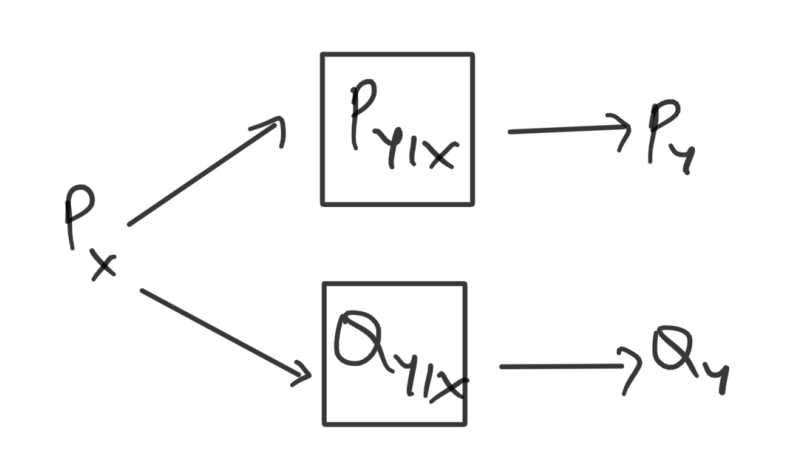
\includegraphics[width=0.3\linewidth]{images/Conditional_Divergence.png}
    \end{figure*}

    \noindent Then $\divergence{P_Y}{Q_Y}\le \divergence{P_\YgX}{Q_\YgX |P_X}$, with equality iff $\divergence{P_{X|Y}}{Q_{X|Y} |P_Y} = 0$.  
\end{theorem}

\begin{proof}
\begin{align*}
    \divergence{P_{X,Y}}{Q_{X,Y}}  &= \divergence{P_\YgX}{Q_\YgX |P_X} +  \underbrace{\divergence{P_X}{P_X}}_{ = 0} \\
        &= \underbrace{\divergence{P_{X|Y}}{Q_{X|Y} |P_Y}}_{\geq 0}  + \divergence{P_Y}{Q_Y}\\
    \implies \divergence{P_Y}{Q_Y} &\le \divergence{P_\YgX}{Q_\YgX |P_X}.
\end{align*}
\end{proof}

\begin{theorem}[\highlight{DPI for Divergence}]
    Given $P_\YgX, P_X$ and $Q_X$, let $P_Y = P_{Y|X} P_X$ and $Q_Y = P_{Y|X}Q_X$, as represented by the diagram. 
    \begin{figure*}[ht]
        \centering
        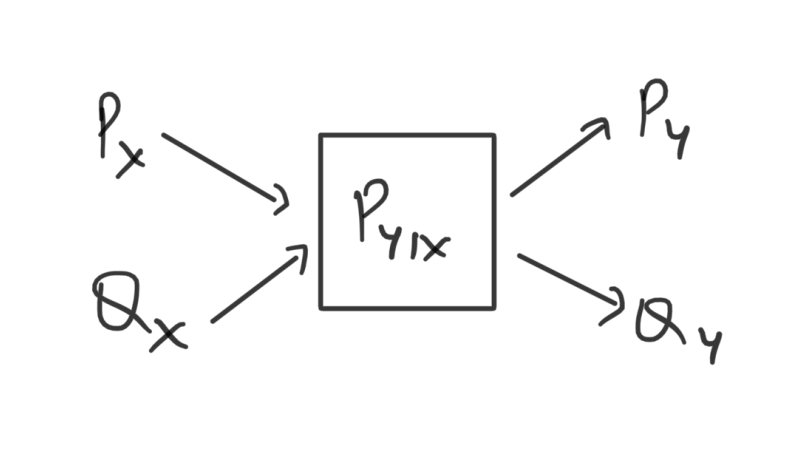
\includegraphics[width=0.3\linewidth]{images/DPI_Divergence.png}
    \end{figure*}

    \noindent Then $\divergence{P_Y}{Q_Y}\le \divergence{P_X}{Q_X}$, with equality iff $\divergence{P_{X|Y}}{Q_{X|Y} |P_Y} = 0$.
\end{theorem}

\begin{proof}
    \begin{align*}
        \divergence{P_{X,Y}}{Q_{X,Y}}  &= \underbrace{\divergence{P_\YgX}{Q_\YgX |P_X}}_{=0} +  \divergence{P_X}{Q_X} \\
            &= \underbrace{\divergence{P_{X|Y}}{Q_{X|Y} |P_Y}}_{\geq 0}  + \divergence{P_Y}{Q_Y}\\
        \implies \divergence{P_Y}{Q_Y} &\le \divergence{P_X}{Q_X}.
    \end{align*}    
\end{proof}

\begin{theorem}
    DPI for Divergence implies DPI for Mutual Information.
\end{theorem}

\begin{proof}
    Now suppose we consider a Markov chain $X - Y - Z$ over discrete random variables. Then notice that 
    \begin{align*}
        P_{Z|X} = P_{Z|X,Y} P_{Y|X} {=} \textcolor{red}{P_{Z|Y}} P_{Y|X}, \quad P_Z = \textcolor{red}{P_{Z|Y}} P_Y.
    \end{align*}
    We apply DPI for divergence on $P_{Z|Y}, P_{Y|X=x}$ and $P_{Y}$ to get
    \begin{align}
        \divergence{P_{Y|X = x}}{P_{Y}}\ \ge \divergence{P_{Z|X = x}}{P_{Z}} \implies &\ \E_X \big[\divergence{P_{Y|X = x}}{P_{Y}}\big]\ \ge \E_X\big[\divergence{P_{Z|X = x}}{ P_{Z}}\big] \nonumber \\
        \implies &\ \divergence{P_{Y|X}}{P_{Y} | P_X}\ \ge \divergence{P_{Z|X}}{ P_{Z} | P_X}.\label{eqn:dpi}
    \end{align}
    Now consider the mutual information
    \begin{align*}
        I(X;Z) &= \divergence{P_{X,Z}}{P_X P_Z} \\
        &= \divergence{P_{Z|X}}{P_Z | P_X} \\
        &\le \divergence{P_{Y|X}}{P_Y | P_X} \tag{using \eqref{eqn:dpi}} \\
        &= \divergence{P_{X,Y}}{P_X P_Y} \\
        &= I(X; Y).
    \end{align*}
\end{proof}

\begin{theorem}[\highlight{Golden Formula}]
    \begin{align*}
        I(X;Y) = \min_{Q_{Y}} \divergence{P_{Y|X}}{Q_{Y}|P_{X}}.
    \end{align*}
\end{theorem}

\begin{proof}
    \begin{align*}
        \divergence{P_{Y|X}}{Q_{Y}|P_{X}} &= \divergence{P_{Y|X}P_{X}}{Q_{Y}P_{X}} \\ 
        &= \sum_{x,y} P_{X,Y} \log{\frac{P_{X,Y}}{Q_{Y}P_{X}} \frac{P_{Y}}{P_{Y}}} \\ 
        &= \sum_{x,y} P_{X,Y} \log{\frac{P_{X,Y}}{P_{X}P_{Y}} + \sum_{x,y} P_{X,Y} \log{\frac{P_{Y}}{Q_{Y}}}} \\ 
        &= \divergence{P_{X,Y}}{P_X P_Y} + \divergence{P_{Y}}{Q_Y} \\ 
        &= I(X;Y) + \divergence{P_{Y}}{Q_Y}.
    \end{align*}
    We get the result by noting that $D(P_{Y}||Q_{Y}) \ge 0$ where equality holds iff $Q_{Y} = P_{Y}.$        
\end{proof}

\begin{definition}
    Let $P$ and $Q$ be two probability mass functions over the same finite (or countably infinite) alphabet $\X$. The \highlight{variational distance} between $P$ and $Q$ is defined as 
    \begin{equation*}
        V(P,Q) = \sum_{x\in\X} \left|P(x) -Q(x)\right|.
    \end{equation*}
\end{definition}

\begin{remark}
    Trivial bounds on variational distance.
\end{remark}

\begin{remark}
    Variational Distance is a Norm.
\end{remark}

\begin{theorem}
    Upper bound of relative entropy in terms of variational distance and entropy.
\end{theorem}

\begin{theorem}[\highlight{Pinsker Inequality}]

\end{theorem}

% \begin{definition}
%     Total Variation Distance.
% \end{definition}

\section{Typicality}

\begin{definition}
    We say that a sequence of random variables $\{X_n\}$ \highlight{converges in probability} to a random variable $X$ if
    \begin{equation*}
        \forall\ \varepsilon > 0, \delta>0, \exists\ N\in\mathbb{Z}_+ \quad \text{such that} \quad  n\ge N \implies \Prob\left[|X_n - X| > \varepsilon \right] < \delta,
    \end{equation*}
    or using the definition of limit, 
    \begin{equation*}
       \lim_{n\rightarrow \infty} \Prob\big[ |X_n - X| > \varepsilon \big] = 0, \quad \varepsilon >0.
    \end{equation*}
\end{definition}

\begin{lemma}[\highlight{Markov Inequality}]
    Let $X$ be a nonnegtaive random variable of finite mean $\E[X]<\infty$. Then for all $a>0$, we have
    \begin{equation*}
        \Prob[X\ge a] \le \dfrac{\E[X]}{a},\quad a > 0.
    \end{equation*}
\end{lemma}

\begin{proof}
    Fix some $a > 0$ and define 
    \begin{equation*}
        Y_a = \begin{cases}
            0\quad\text{if } X<a, \\
            a\quad\text{if } X\ge a.
        \end{cases}
    \end{equation*}
    Since $X$ is nonnegative by assumption, it follows that $Y_a \le X$ or equivalently $\E[Y_a] \le \E[X]$. On other hand, we have
    \begin{equation*}
        \E[Y_a] = a \Prob[X \ge a] \implies \Prob[X\ge a] \le \dfrac{\E[X]}{a}. 
    \end{equation*}
\end{proof}

\begin{lemma}[\highlight{Chebyshev Inequality}]
    Let $X$ be a random variable with finite mean and finite variance. Then for all $\varepsilon>0$, we have
    \begin{equation*}
        \Prob[|X-\E[X]|\ge \varepsilon] \le \dfrac{\Var[X]}{\varepsilon^2},\quad \varepsilon > 0.
    \end{equation*}
\end{lemma}

\begin{proof}
    This follows directly from applying the Markov Inequality to $(X-\mu)^2$ with $a = \varepsilon^2$. 
\end{proof}

\begin{lemma}[\highlight{Weak Law of Large Numbers}]
    Let $\{Z_n\}$ be a sequence of independent and identically distributed (i.i.d.) random variables with mean $\mu$ an variance $\sigma^2$. Let 
    \begin{equation*}
        S_n = \dfrac{1}{n}\sum_{k=1}^n Z_k
    \end{equation*}
    be the sample mean. Then $\{S_n\}$ converges in probability to $\mu$. In particular, 
    \begin{equation*}
        \Prob[|S_n-\mu|\ge \varepsilon] \le \dfrac{\sigma^2}{n\varepsilon^2},\quad \varepsilon > 0.
    \end{equation*}
\end{lemma}

\begin{proof}
    Observe that 
    \begin{gather*}
        \E[S_n] = \dfrac{1}{n}\sum_{k=1}^n \E\left[ Z_k \right] = \mu, \\
        \Var\left(\dfrac{Z_k}{n}\right) = \E\left[\left( \dfrac{Z_k}{n} - \E\left[ \dfrac{Z_k}{n} \right]\right)^2 \right] = \E\left[\left( \dfrac{Z_k}{n} - \dfrac{\mu}{n} \right)^2\right] = \dfrac{\E\left[\left( Z_k - \mu \right)^2\right]}{n^2} = \dfrac{\sigma^2}{n^2}, \\
        \Var(S_n) = \sum_{k=1}^{n} \Var\left(\dfrac{Z_k}{n}\right) = \dfrac{\sigma^2}{n},
    \end{gather*}
    where we used the property that variance of sum of i.i.d.~random variables is sum of variance of each random variable.

    By applying Chebyshev Inequality on $S_n$ for some $\varepsilon > 0$, we get the required bound on tail probability. The convergence of $S_n$ is a direct consequence of setting $N = 1$ in the tail bound for all $\varepsilon > 0$.
\end{proof}

\begin{definition}[\highlight{Type}]
    Let $x^{(n)}$ be a sequence of $n$ elements drawn from a finite-cardinality alphabet $\mathcal{X}$. The \highlight{empirical probability mass function} of $x^{(n)}$, also referred to as its \highlight{type}, is defined for $x\in \mathcal{X}$ as
    \begin{equation*}
        \pi(x|x^{(n)}) = \dfrac{|\{i\in [n]\;:\;x_i = x\}|}{n}, 
    \end{equation*}
    where $[n] = \{1,\ldots, n\}$.
\end{definition}

\begin{theorem}
    Let $\{X_n\}$ be an i.i.d.~sequence of random variables with $X_i\sim P_X$. Then $\forall\ x\in\mathcal{X}$ and for all $\varepsilon>0$, we have
    \begin{equation*}
        \lim_{n\rightarrow \infty} \Prob[|\pi(x|X^{(n)}) - P_X(x)| \ge \varepsilon] = 0, 
    \end{equation*}
    or in other words, $\{\pi(x|X^{(n)})\}$ converges in probability to $P_X(x)$ for all $x\in\mathcal{X}$.
\end{theorem}

\begin{proof}
    We can rewrite empirical pmf as 
    \begin{equation*}
        \pi(x|X^{(n)}) = \sum_{k=1}^{n} \dfrac{\mathbb{I}_{[X_k =\, x]}}{n}, 
    \end{equation*}
    where $\mathbb{I}$ is the indicator function. Notice that
    \begin{align*}
        \E\left[\mathbb{I}_{[X_k =\, x]}\right] &= P_X(x), \\
        \Var\left[ \mathbb{I}_{[X_k =\, x]} \right] &= \E\left[\left( \mathbb{I}_{[X_k =\, x]} \right)^2\right] - \left(\E\left[\mathbb{I}_{[X_k =\, x]}\right]\right)^2 \\
        &= P_X(x) - P_X(x)^2 \\ 
        &= P_X(x)(1-P_X(x)).
    \end{align*}
    Applying Weak Law of Large Numbers on $\{\pi(x|X^{(n)})\}$, we get 
    \begin{equation*}
        \Prob[|\pi(x|X^{(n)}) - P_X(x)|\ge \varepsilon] \le \dfrac{P_X(x)(1-P_X(x))}{n\varepsilon^2}.
    \end{equation*}
\end{proof}

\begin{definition}[\highlight{Typical Set}]
    The {set of $\varepsilon$-typical $n$-sequences} (simply typical set) for a random variable $X\sim P_X$, $n\in\mathbb{Z}_+$ and $\varepsilon \in (0,1)$ is defined as
    \begin{equation*}
        \T^{(n)}_\varepsilon (X) = \{x^{(n)}\;:\; |\pi(x|x^{(n)}) - P_X(x)| \le \varepsilon P_X(x), \forall\ x\in\mathcal{X}\}.
    \end{equation*}
\end{definition}

\begin{remark}
    For an element $x\in\mathcal{X}$ which has $P_X(x) = 0$ cannot be a part of typical sequence. To see why, suppose on contrary such an $x$ belonged to a sequence $x^{(n)}$, then $\pi(x|x^{(n)}) > 0$. Consequently, we have $|\pi(x|x^{(n)}) - P_X(x)| = \pi(x|x^{(n)}) > 0 = \varepsilon P_X(x)$ for all $\varepsilon > 0$, which shows that $x^{(n)}$ is not a typical sequence.
\end{remark}

\begin{lemma}[\highlight{Typical Average Lemma}]
    Consider a typical sequence $x^{(n)}\in \T^{(n)}_\varepsilon (X)$. Then for any {nonnegtaive} function $\mapping{g}{\X}{\R}$, we have 
    \begin{equation*}
        (1-\varepsilon) \E[g(X)] \le \dfrac{1}{n} \sum_{k=1}^{n} g(x_k) \le (1+\varepsilon) \E[g(X)].
    \end{equation*}
\end{lemma}

\begin{proof}
    Since $x^{(n)}\in\T^{(n)}_\varepsilon$, we have
    \begin{equation*}
        (1-\varepsilon) P_X(x) \le \pi(x|x^{(n)}) \le (1+\varepsilon) P_X(x).
    \end{equation*}
    Summing the above inequality over $\X$ and multiplying by $g(x)$, we get 
    \begin{align*}
        \sum_{x\in\X} (1-\varepsilon) P_X(x) g(x) &\le \sum_{x\in\X} \pi(x|x^{(n)}) g(x) \le \sum_{x\in\X} (1+\varepsilon) P_X(x) g(x) \\
        \implies (1-\varepsilon) \E[g(X)] &\le \sum_{x\in\X} \pi(x|x^{(n)}) g(x) \le (1+\varepsilon) \E[g(X)],
    \end{align*} 
    where we used the nonnegativity of $g$ to retain the inequality on mutliplication. We obtain the result by noting that
    \begin{equation*}
        \sum_{x\in\X} \pi(x|x^{(n)}) g(x) = \dfrac{1}{n} \sum_{k=1}^n g(x_k),
    \end{equation*}
    where $x_k$ is the $k$-th element of the sequence $x^{(n)}$.
\end{proof}

\begin{theorem}[\highlight{Properties of Typical Sequence}]\label{thm:typicality}
    Let $X^{(n)}$ have i.i.d.~entries with $X_i\sim P_X$ and suppose $\varepsilon>0$.
    \begin{enumerate}[(a)]
        \item All typical sequences are essentially equiprobable: If $x^{(n)}\in\T^{(n)}_\varepsilon(X)$, then 
        \begin{equation*}
            2^{-n(1+\varepsilon)H(X)} \le \Prob[x^{(n)}] \le 2^{-n(1-\varepsilon)H(X)},
        \end{equation*}
        where we define $\Prob[x^{(n)}] = \prod_{i=1}^{n} P_X(x_i)$.
        \item Almost all probability mass is in the typical set: 
        \begin{equation*}\label{eqn:not_in_typical_set}
            \Prob\left[ X^{(n)} \notin \T^{(n)}_\varepsilon \right] \le \left(\dfrac{1}{n}\right).
        \end{equation*}
        \item Bounds on cardinality of typical set:
        \begin{equation*}\label{eqn:typical_set_cardinality}
            \left(1-\dfrac{1}{n}\right) 2^{n(1-\varepsilon)H(X)} \le \left| \T^{(n)}_\varepsilon \right| \le 2^{n(1+\varepsilon)H(X)}.
        \end{equation*}
    \end{enumerate}
\end{theorem}

% \begin{proof}
%     \textbf{(a)}

%     \noindent \textbf{(b)}

%     \noindent \textbf{(c)}
% \end{proof}

\section{Lossless Source Coding}

\begin{problem*}[Refer Fig. \ref{fig:Source_Coding}]
    The source sequence $X^{(n)}$ is encoded into an index $M$ at rate $R$ bits per source symbol, and the receiver decodes the index to find the estimate $\hat{X}^{(n)}$ of the source sequence. The lossless source coding problem is to find the lowest compression rate in bits per source symbol such that the probability of decoding error decays asymptotically to zero with the code block length $n$.
\end{problem*}

\begin{figure}[ht]
    \centering
    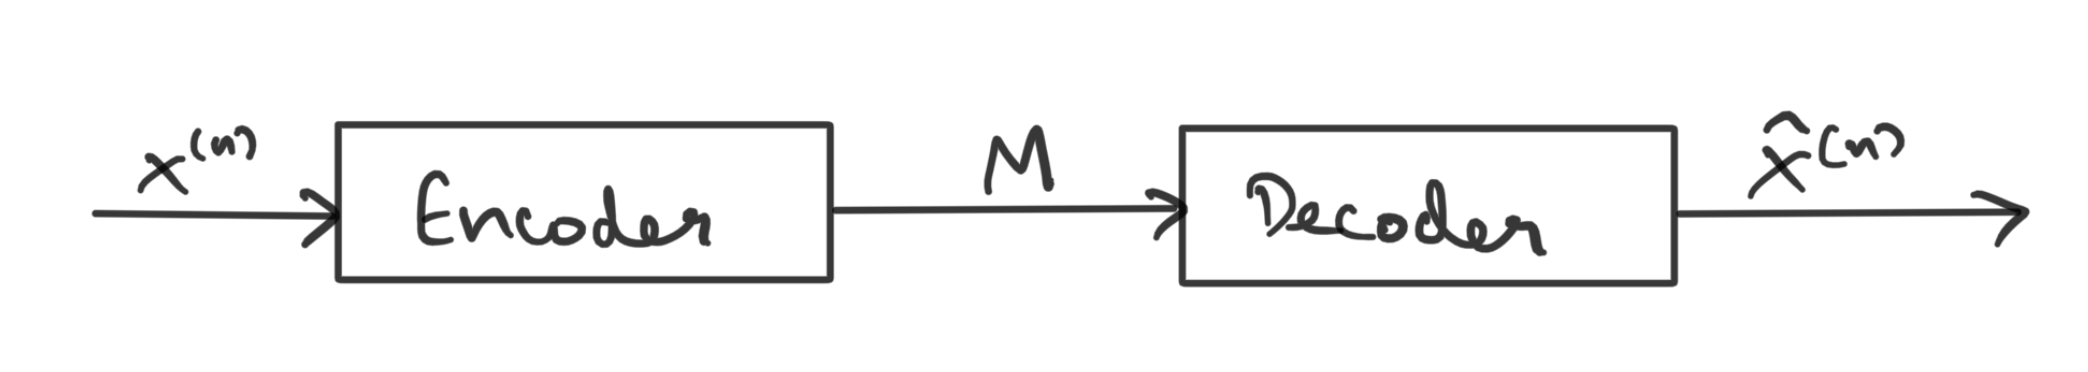
\includegraphics[width=0.7\linewidth]{images/Source_Coding.png}
    \caption{Point-to-point compression system.}
    \label{fig:Source_Coding}
\end{figure}

\begin{definition}
    A \highlight{discrete memoryless source (DMS)}, denoted by $(\X,P_X)$ and informally referred to as $X$, consists of
    \begin{itemize}
        \item a finite alphabet $\X$ and 
        \item a probability mass function $P_X$ over $\X$.
    \end{itemize}
    The source is \textit{stationary} and \textit{memoryless} in the sense that it is time-invariant and generates i.i.d.~random symbols $\{X_i\}$ with $X_i\sim P_X$.
\end{definition}

\begin{remark}
    The prefix ``discrete memoryless'' refers to ``finite-alphabet, time-invariant and memoryless''.
\end{remark}

% \begin{remark}
%     It turns out that to compress the source effectively, we need to group source symbols in blocks, and perform processing block by block. Specifically, our scheme will map a block of $n$ source symbols into an index belonging to a set $\M$ of cardinality $|\M|$. Note that we need $\log_2 |\M|$ bits to save each index. The rate $R$ of such a fixed-length
%     source code is $R = \log_2 |\M|n$ bits per source symbol. 
% \end{remark}

% \begin{remark}
%     It turns out convenient to specify a family of fixed-length source codes with rate $R$, parameterized with respect to the number of symbols $n$ in each block. If we keep $R$ fixed, then the cardinality of the message set $\M$ needs to grow exponentially in $n$ as $2^{nR}$.
% \end{remark}

\begin{definition}
    A $(2^{nR},n)$ \highlight{lossless source code} of rate $R$ bits per source symbol consists of 
    \begin{itemize}
        \item an encoder $\mapping{m}{\X^n}{[2^{nR}]}$ that assigns an index $m(x^{(n)})$, a codeword of length $nR$ bits, to each source $n$-sequence $x^{(n)}$, and
        \item a decoder $\mapping{\hat{x}^{(n)}}{[2^{nR}]}{\X^{n}\cup \{e\}}$ that assigns an estimate $\hat{x}^{(n)}(m)\in\X^n$ or an error message $e$ to each index $m\in[2^{nR}]$.
    \end{itemize}
\end{definition}

\begin{definition}
    The \highlight{probability of decoding error} for a $(2^{nR}, n)$ lossless source code is defined as $P^{(n)}_e = \Prob[\hat{X}^{(n)}\neq X^n]$. A rate $R$ is said to be \highlight{achievable} if there exists a sequence of $(2^{nR}, n)$ codes such that $\lim_{n\rightarrow \infty} P_e^{(n)} = 0$. The \highlight{optimal rate} $R^*$ for lossless source coding is the infimum of all achievable rates.
\end{definition}

\begin{remark}
    The lossless source coding scheme is required to be only asymptotically error-free (lossless).
\end{remark}

\begin{theorem}[\highlight{Fano's Inequality}]
    Let $X, Y$ be two random variables on $\X$ such that $\hat{X}$ is an estimator of $X$ and $X - Y - \hat{X}$. Let the error probability be defined as $P_e = \Prob[X \neq \hat{X}]$. Then 
    \begin{equation*}
        H(X|Y) \le H(X|\hat{X}) \le H_b(P_e) + P_e log(|\X|-1) \le 1 + P_e log|\X|. 
    \end{equation*}
\end{theorem}

\begin{proof}
    Define the indicator random variable 
    \begin{equation*}
        Z = \begin{cases}
            1\quad\text{if } \hat{X}\neq X,\\
            0\quad\text{if } \hat{X} = X.
        \end{cases}
    \end{equation*}
    Then $P_Z(1) = P_e$ and $H(Z) = H_b(P_e)$. Now we use the chain rule to derive the following:
    \begin{align*}
        H(X,Z|\hat{X}) &= H(X|\hat{X}) + \underbrace{H(Z|X,\hat{X})}_{=0} \\
        &= H(Z|\hat{X}) + H(X|\hat{X},Z) \\
        &\le H(Z) + H(X|\hat{X},Z) \\
        &= H_b(P_e) + P_Z(0)\underbrace{H(X|\hat{X},Z = 0)}_{=0} + P_Z(1)H(X|\hat{X},Z = 1) \\
        &\le H_b(P_e) + P_e\log(|\X|-1) \tag{since $X\neq\hat{X}$} \\
        \implies H(X|\hat{X}) &\le H_b(P_e) + P_e\log(|\X|-1).
    \end{align*}
    The upper bound is obtained by upper bounding $H_b(P_e)$ and $\log(|\X|-1)$. Using the DPI for mutual information, we get the lower bound.
\end{proof}

\begin{theorem}[\highlight{Lossless Source Coding Theorem}] 
    The optimal rate for lossless source coding of a discrete memoryless source $X$ is 
    \begin{equation*}
        R^* = H(X).
    \end{equation*}
\end{theorem}

\begin{proof}[Proof Sketch]\renewcommand{\qedsymbol}{}
    To prove this theorem, we need to verify the following two statements:
    \begin{itemize}
        \item \textbf{Achievability.} For every $R > R^* = H(X)$ there exists a sequence of $(2^{nR}, n)$ codes with $\lim_{n\rightarrow \infty} P_e^{(n)} = 0$.
        \item \textbf{Converse.} For every sequence of $(2^{nR}, n)$ codes with $\lim_{n\rightarrow \infty} P_e^{(n)} = 0$, the source coding rate $R \ge R^* = H(X)$.
    \end{itemize}
\end{proof}

\begin{proof}
    \textbf{(Achievability).} For $\varepsilon > 0$, let $R = (1+\varepsilon)H(X)$.  So for a given $n$ our coding scheme maps $n$ symbols into a $\M$ such that $|\M| = 2^{nR} = 2^{n(1+\varepsilon)H(X)}$. By the upper bound on the cardinality of the typical set in Thm. \ref{thm:typicality} \eqref{eqn:typical_set_cardinality}, we can uniquely map each typical sequence in $\T^{(n)}_\varepsilon$ to an index in $\M$. Therefore, we define the typicality coding scheme:
    \begin{itemize}
        \item {(Encoding).} Assign a unique index $m(x^{(n)})$ to each $x^{(n)}\in\T^{(n)}_\varepsilon$. Assign $m = 1$ to all $x^{(n)}\notin \T^{(n)}_\varepsilon$. 
        \item {(Decoding).} Upon receiving the index $m$, the decoder returns the typical sequence corresponding to $m$, i.e., return $\hat{x}^{(n)} = x^{(n)}(m)$ for the unique $x^{(n)}(m)\in\T^{(n)}_\varepsilon$.
    \end{itemize}

    \noindent All typical sequences are recovered error-free. Thus, $P^{(n)}_\varepsilon = \Prob[X^{(n)}\notin\T^{(n)}_\varepsilon]$ which vanishes to zero as $n\rightarrow \infty$ by Thm. \ref{thm:typicality} \eqref{eqn:not_in_typical_set}. This completes the achievability proof.

    \noindent \textbf{(Converse).} Given a sequence of $(2^{nR},n)$ codes with $\lim_{n\rightarrow \infty} P^{(n)}_\varepsilon = 0$, let $M$ be a random variable corresponding to the index generated by the encoder. Note that $X^{(n)} - M - \hat{X}^{(n)}$ forms a Markov chain, by Fano's Inequality, we have
    \begin{equation*}
        H(X^{(n)}|M) \le H(X^{(n)}|\hat{X}^{(n)}) \le 1 + P_e \log|\X^n|\le 1 + nP_e\log|\X|.
    \end{equation*}
    Now consider 
    \begin{align*}
        nR &\ge H(M) \\
        &= I(M;X^{(n)})\tag{since $H(X^{(n)}|M) = 0$} \\
        &= nH(X) - H(X^{(n)}|M) \\
        &\ge nH(X) - 1 - nP_e\log|\X|\\
        \implies R &\ge H(X) - \dfrac{1}{n} - P^{(n)}_\varepsilon\log|\X|.
    \end{align*}
    By taking $n\rightarrow \infty$, we conclude that $R\ge H(X)$.
\end{proof}

\section{Joint Typicality}

\begin{definition}[\highlight{Joint Type}]
    Let $(x^{(n)}, y^{(n)})$ be a pair of $n$ length sequences from a finite-cardinality alphabet $(\mathcal{X},\mathcal{Y})$. The {joint empirical probability mass function} of $(x^{(n)}, y^{(n)})$, also referred to as its {joint type}, is defined for $(x,y)\in \X\times \Y$ as
    \begin{equation*}
        \pi(x,y|x^{(n)}, y^{(n)}) = \dfrac{|\{i\in [n]\;:\;(x_i,y_i) = (x,y)\}|}{n}.
    \end{equation*}
\end{definition}

\begin{remark}
    The $X$-marginal of $X,Y$-joint empirical probability mass function is the $X$-empirical probability mass function and similarly for $Y$, i.e.,
    \begin{equation*}
        \sum_{y\in\Y} \pi(x,y|x^{(n)},y^{(n)}) = \pi(x|x^{(n)}),\qquad \sum_{x\in\X} \pi(x,y|x^{(n)},y^{(n)}) = \pi(y|y^{(n)}).
    \end{equation*}
\end{remark}

\begin{definition}[\highlight{Jointly Typical Set}]
    The {set of $\varepsilon$-jointly typical $n$-sequences}, simply jointly typical set, for a random variable $(X,Y)\sim (P_X,P_Y)$ and $\varepsilon \in (0,1)$ is defined as
    \begin{equation*}
        \mathcal{T}^{(n)}_\varepsilon (X,Y) = \{(x^{(n)},y^{(n)})\;:\; |\pi(x,y|x^{(n)},y^{(n)}) - P_{X,Y}(x,y)| \le \varepsilon P_{X,Y}(x,y), \forall\ x\in\mathcal{X}, y\in\mathcal{Y}\}.
    \end{equation*}
\end{definition}

\begin{theorem}[\highlight{Marginal Typicality}]
    Let $(x^{(n)},y^{(n)})\in \mathcal{T}_\varepsilon^{(n)}(X,Y)$ and $P(x^{(n)}, y^{(n)}) = \prod_{i=1}^{n}P_{X,Y}(x_i,y_i)$. Then
    \begin{enumerate}[(a)]
        \item $x^{(n)}\in\T^{(n)}_\varepsilon(X)$ and $y^{(n)}\in \T^{(n)}_\varepsilon(Y)$,
        \item $P(x^{(n)}) \overset{\circ}{=} 2^{-nH(X)}$ and $P(y^{(n)}) \overset{\circ}{=} 2^{-nH(Y)}$,
        \item $P(x^{(n)}|y^{(n)}) \overset{\circ}{=} 2^{-nH(X|Y)}$ and $P(y^{(n)}|x^{(n)}) \overset{\circ}{=} 2^{-nH(Y|X)}$,
        \item $P(x^{(n)},y^{(n)}) \overset{\circ}{=} 2^{-nH(X,Y)}$,
        \item $2^{n(1-\varepsilon)H(X,Y)} \le |\T^{(n)}_\varepsilon(X,Y)| \le 2^{n(1+\varepsilon)H(X,Y)}$,
    \end{enumerate}
    where we define $P(\cdot) \overset{\circ}{=} 2^{-nH(\cdot)}$ to be $2^{-n(1+\varepsilon)H(\cdot)} \le P(\cdot) \le 2^{-n(1-\varepsilon)H(\cdot)}$.
\end{theorem}

\begin{proof}
    \textbf{(a)} Observe that 
    \begin{align*}
        (1-\varepsilon) P_{X,Y}(x,y) \le \pi(x,y&|x^{(n)},y^{(n)}) \le (1+\varepsilon) P_{X,Y}(x,y) \\
        \implies \sum_{y\in\Y}(1-\varepsilon)  P_{X,Y}(x,y) \le \sum_{y\in\Y} \pi(x,y&|x^{(n)},y^{(n)}) \le \sum_{y\in\Y} (1+\varepsilon) P_{X,Y}(x,y) \\ 
        \implies (1-\varepsilon) P_{X}(x) \le \pi(x&|x^{(n)}) \le (1+\varepsilon) P_{X}(x),
    \end{align*}
    in other words, $x^{(n)}\in\T^{(n)}_\varepsilon(X)$. Similarly, $y^{(n)}\in \T^{(n)}_\varepsilon(Y)$.

    % \noindent \textbf{(b)}

    % \noindent \textbf{(c)}
    
    % \noindent \textbf{(d)}
    
    % \noindent \textbf{(e)}
\end{proof}

\begin{theorem}[\highlight{Conditional Typicality Lemma}]
    Let $(X,Y)\sim P_{X,Y}$. Suppose $x^{(n)}\in\T^{(n)}_\varepsilon(X)$ and $Y^{(n)}\sim P_{Y^{(n)}|X^{(n)} =\,x^{(n)}} = \prod_{i=1}^{n} P_{Y|X =\, x_i}$. Then, for every $\varepsilon > \varepsilon^\prime$,
    \begin{equation*}
        \lim_{n\rightarrow\infty} \Prob[(x^{(n)},Y^{(n)})\in\T^{(n)}_\varepsilon(X,Y)] = 1.
    \end{equation*}
\end{theorem}

\begin{remark}[\highlight{Need for both $\varepsilon$ and $\varepsilon^\prime$}]
    Let $(X,Y)$ be a pair of independent Bern$(1/2)$ random variables. Let $k = \lfloor (n/2)(1+\varepsilon) \rfloor$ and $x^{(n)}$ be a binary sequence with $k$ ones followed by $(n-k)$ zeros. Then $x^{(n)}\in \T^{(n)}_\varepsilon(X)$. Let $Y^{(n)}$ be an i.i.d.~Bern$(1/2)$ sequence, independent of $x^{(n)}$. Then 
    \begin{equation*}
        \Prob[(x^{(n)},Y^{(n)})\in\T^{(n)}_\varepsilon(X,Y)] \le \Prob\left[ \sum_{i=1}^k Y_i < (k+1)/2 \right] \overset{n\rightarrow \infty}{\longrightarrow} \dfrac{1}{2}.
    \end{equation*}
    Thus, the fact that $x^{(n)}\in\T^{(n)}_\varepsilon(X)$ and $Y^{(n)}\sim P_{Y^{(n)}|X^{(n)}=\,x^{(n)}}$ does not necessarily imply that $\Prob[(x^{(n)},Y^{(n)})\in\T^{(n)}_\varepsilon(X,Y)]$.
\end{remark}

\begin{theorem}[\highlight{Conditionally Typical Set}]
    Let $(X,Y)\sim P_{X,Y}$ and define 
    \begin{equation*}
        \T^{(n)}_\varepsilon(Y|x^{(n)}) = \{y^{(n)}\;:\; (x^{(n)},y^{(n)})\in\T^{(n)}_\varepsilon(X,Y)\}.
    \end{equation*}
    Then for every $x^{(n)}\in \X^n$,
    \begin{equation*}
        |\T^{(n)}_\varepsilon (Y|x^{(n)})| \le 2^{n(H(Y|X)+\delta(\varepsilon))}
    \end{equation*}
    for some $\delta(\varepsilon) \rightarrow 0$ and $\varepsilon \rightarrow 0$. Additionally, if $x^{(n)}\in \T^{(n)}_{\varepsilon^\prime}(X)$ with $\varepsilon^\prime < \varepsilon$, then 
    \begin{equation*}
        |\T^{(n)}_\varepsilon (Y|x^{(n)})| \ge [1-\mathcal{O}(1/n)] 2^{n(H(Y|X)-\delta(\varepsilon))}, \quad n\rightarrow \infty.
    \end{equation*}
\end{theorem}

\begin{remark}
    The upper bound on the conditionally typical set holds for every $x^{(n)}\in\X^n$ and not just for $x^{(n)}\in \T^{(n)}_{\varepsilon}(X)$.
\end{remark}

\begin{theorem}[\highlight{Joint Typicality Lemma}]
    Let $(X,Y)\sim P_{X,Y}$. Suppose $x^{(n)}\in\T^{(n)}_{\varepsilon^\prime}(X)$ and $\bar{Y}^{(n)}\sim P_{\bar{Y}^{(n)}} = \prod_{i=1}^{n} P_{Y}$ (instead of $\prod_{i=1}^{n} P_{Y|X =\,x_i}$). Then, for every $\varepsilon > \varepsilon^\prime$,
    \begin{equation*}
        (1-\mathcal{O}(1/n))2^{-n(I(X;Y)+\delta(\varepsilon))} \le \Prob[(x^{(n)}, \bar{Y}^{(n)})\in\T^{(n)}_\varepsilon(X,Y)] \le 2^{-n(I(X;Y)-\delta(\varepsilon))},
    \end{equation*}
    where $\delta(\varepsilon) \rightarrow 0$ as $\varepsilon \rightarrow 0$. Furthermore, let $\bar{X}^{(n)} \sim P_{\bar{X}^{(n)}} = \prod_{i=1}^{n} P_{X}$ and $\bar{Y}^{(n)}\sim P_{\bar{Y}^{(n)}} = \prod_{i=1}^{n} P_{Y}$. Then 
    \begin{equation*}
        \Prob[(\bar{X}^{(n)}, \bar{Y}^{(n)})\in\T^{(n)}_\varepsilon(X,Y)] \le 2^{-n(I(X;Y)-\delta(\varepsilon))},
    \end{equation*}
    where $\delta(\varepsilon) \rightarrow 0$ as $\varepsilon \rightarrow 0$.
\end{theorem}

\section{Channel Coding}

\begin{problem*}[Refer Fig. \ref{fig:Channel_Coding}]
    The sender encodes the message $M$ into a codeword $X^{(n)}$ and transmits it over the channel in $n$ time instances. Upon receiving the
    noisy sequence $Y^{(n)}$, the receiver decodes it to obtain the estimate $\hat{M}$ of the message. The channel coding problem is to find the channel capacity, which is the highest rate $R$ such that the probability of decoding error can be made to decay asymptotically to zero with
    the code block length $n$.
\end{problem*}

\begin{figure}[ht]
    \centering
    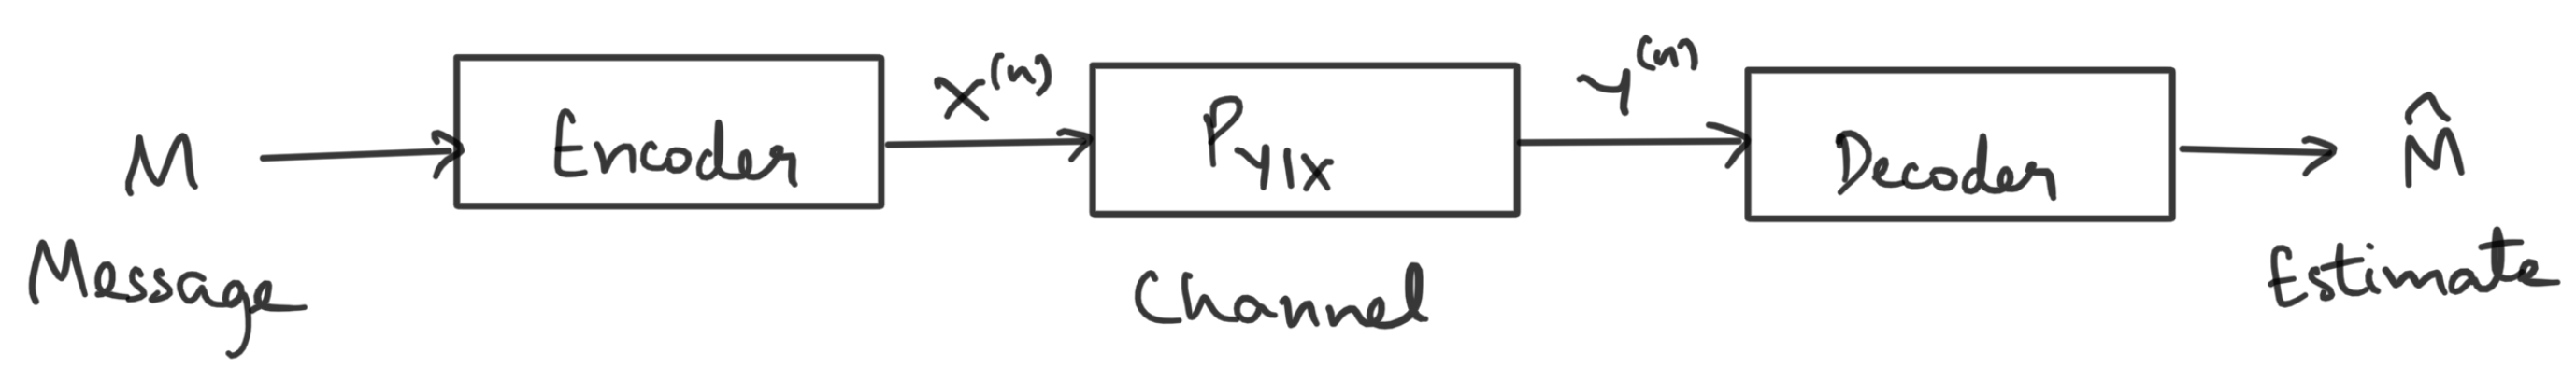
\includegraphics[width=\linewidth]{images/Channel_Coding.png}
    \caption{Point-to-point communication system.}
    \label{fig:Channel_Coding}
\end{figure}

\begin{definition}
    A \highlight{discrete memoryless channel (DMC)}, denoted by $(\X,P_{Y|X},\Y)$ and informally referred to as $P_{Y|X}$, consists of
    \begin{itemize}
        \item a finite input alphabet $\X$,
        \item a finite output alphabet $\Y$ and
        \item a collection of conditional probability mass functions $P_{Y|X = x}$ over $\Y$ for every $x\in\X$. 
    \end{itemize}
    The channel is \textit{stationary} (time-invariant) and \textit{memoryless} in the sense that when it is used $n$ times with message $M$ drawn from an arbitrary set and input $X^{(n)}\in\X^n$, the output $Y_i\in\Y$ at time $i\in[n]$ given $(M,X^{(i)},Y^{(i-1)})$ is distributed according to 
    \begin{equation*}
        P_{Y_i|X^{(i)},Y^{(i-1)},M}(y_i|x^{(i)},y^{(i-1)},m) = P_{Y|X}(y_i|x_i),\quad i\in[n].
    \end{equation*}
    Equivalently, memoryless property induces the following Markov chain:
    \begin{equation*}
        (X^{(i-1)},Y^{(i-1)},M) - X_i - Y_i.
    \end{equation*}
\end{definition}

\begin{definition}
    A $(2^{nR},n)$ \highlight{channel coding scheme} (simply code) for a DMC $(\X,P_{Y|X},\Y)$ consists of 
    \begin{itemize}
        \item a message set $[2^{nR}]$,
        \item an encoder $\mapping{m}{[2^{nR}]}{\X^n}$ that assigns a codeword $x^{(n)}(m)$ to each $m\in[2^{nR}]$, and
        \item a decoder $\mapping{\hat{m}}{\Y^n}{{[2^{nR}]}\cup \{e\}}$ that assigns an estimate $\hat{m}\in[2^{nR}]$ or an error message $e$ to each received sequence $y^{(n)}$.
    \end{itemize}
\end{definition}

\begin{definition}
    We say that a DMC is used \highlight{without feedback} if 
    \begin{equation*}
        P_{X_i|X^{(i-1),Y^{(i-1)}},M}(x_i|x^{(i-1)},y^{(i-1)},m) = P_{X_i|X^{(i-1)}}(x_i|x^{(i-1)}),\quad i\in[n].
    \end{equation*}
\end{definition}

\begin{lemma}
    If a DMC is used without feedback, then 
    \begin{equation*}
        P_{Y^{(n)}|X^{(n)},M}(y^{(n)}|x^{(n)},m) = \prod_{i=1}^{n} P_{Y|X}(y_i|x_i),\quad \forall\ n\ge 1.
    \end{equation*}
    Equivalently, no feedback induces $Y_i - (M,X^{(i)}) - X^{(i+1:n)}$.
\end{lemma}

\begin{proof}
    Consider the following joint distribution
    \begin{align*}
        &P_{X^{(n)},Y^{(n)},M}(x^{(n)},y^{(n)},m) \\
        &\quad = P_M(m) \prod_{i=1}^{n} P_{X_i|X^{(i-1)},Y^{(i-1)},M}(x_i|x^{(i-1)},y^{(i-1)},m) P_{Y_i|X^{(i)},Y^{(i-1)},M}(y_i|x^{(i)},y^{(i-1)},m) \\
        &\quad = P_M(m) \prod_{i=1}^{n} P_{X_i|X^{(i-1)},M}(x_i|x^{(i-1)},m) P_{Y|X}(y_i|x_i) = P_{X^{(n)},M}(x^{(n)},m) \prod_{i=1}^{n} P_{Y|X}(y_i|x_i).
    \end{align*}
    But, $P_{X^{(n)},Y^{(n)},M}(x^{(n)},y^{(n)},m) = P_{X^{(n)},M}(x^{(n)},m) P_{Y^{(n)}|X^{(n)},M}(y^{(n)}|x^{(n)},m)$.
\end{proof}

\begin{assume}\label{assume:channel_coding}
    The message is uniformly distributed over the message set, i.e., $P_M(m) = \dfrac{1}{2^{nR}}$.
\end{assume}

\begin{definition}
    The set $\C = \{x^{(n)}(1),x^{(n)}(2),\ldots,x^{(n)}(2^{nR})\}$, which is the set of all codewords, is referred to as the \highlight{codebook} associated with the $(2^{nR},n)$ code. Define $\lambda_m(\C)$ to be the conditional probability of error given that message $m$ is sent, i.e.,
    \begin{equation*}
        \lambda_m(\C) = \Prob[\hat{M}\neq m | M = m] = \sum_{y^{(n)}\in\Y^n} P_{Y^{(n)}|X^{(n)}}(y^{(n)}|x^{(n)}(m)) \mathbb{I}_{[\hat{m}(y^{(n)})\neq\, m]}.
    \end{equation*}
    Then the \highlight{average probability of error} for a $(2^{nR}, n)$ code is defined as 
    \begin{equation*}
        P^{(n)}_e(\C) = \Prob[\hat{M}\neq M] = \dfrac{1}{2^{nR}} \sum_{m=1}^{2^{nR}} \lambda_m(\C).   
    \end{equation*}
    A rate $R$ is said to be \highlight{achievable} if there exists a sequence of $(2^{nR}, n)$ codes such that $\lim_{n\rightarrow \infty} P_e^{(n)} = 0$. The \highlight{capacity} $C$ of a DMC is the supremum of all achievable rates.
\end{definition}

\begin{theorem}[\highlight{Channel Coding Theorem}]
    Under Assumption \ref{assume:channel_coding}, the capacity of the DMC $(\X,P_{Y|X},\Y)$ without feedback is given by
    \begin{equation*}
        C = \max_{P_X}\,I(X;Y).
    \end{equation*}
\end{theorem}

% \begin{proof}[Proof Sketch]\renewcommand{\qedsymbol}{}
%     To prove this theorem, we need to verify the following two statements:
%     \begin{itemize}
%         \item \textbf{Achievability.} For every $R > R^* = H(X)$ there exists a sequence of $(2^{nR}, n)$ codes with $\lim_{n\rightarrow \infty} P_e^{(n)} = 0$.
%         \item \textbf{Converse.} For every sequence of $(2^{nR}, n)$ codes with $\lim_{n\rightarrow \infty} P_e^{(n)} = 0$, the source coding rate $R \ge R^* = H(X)$.
%     \end{itemize}
% \end{proof}

% \begin{proof}
%     \textbf{(Achievability).} For $\varepsilon > 0$, let $R = (1+\varepsilon)H(X)$.  So for a given $n$ our coding scheme maps $n$ symbols into a $\M$ such that $|\M| = 2^{nR} = 2^{n(1+\varepsilon)H(X)}$. By the upper bound on the cardinality of the typical set in Thm. \ref{thm:typicality} \eqref{eqn:typical_set_cardinality}, we can uniquely map each typical sequence in $\T^{(n)}_\varepsilon$ to an index in $\M$. Therefore, we define the typicality coding scheme:
%     \begin{itemize}
%         \item {(Encoding).} Assign a unique index $m(x^{(n)})$ to each $x^{(n)}\in\T^{(n)}_\varepsilon$. Assign $m = 1$ to all $x^{(n)}\notin \T^{(n)}_\varepsilon$. 
%         \item {(Decoding).} Upon receiving the index $m$, the decoder returns the typical sequence corresponding to $m$, i.e., return $\hat{x}^{(n)} = x^{(n)}(m)$ for the unique $x^{(n)}(m)\in\T^{(n)}_\varepsilon$.
%     \end{itemize}

%     \noindent All typical sequences are recovered error-free. Thus, $P^{(n)}_\varepsilon = \Prob[X^{(n)}\notin\T^{(n)}_\varepsilon]$ which vanishes to zero as $n\rightarrow \infty$ by Thm. \ref{thm:typicality} \eqref{eqn:not_in_typical_set}. This completes the achievability proof.

%     \noindent \textbf{(Converse).} Given a sequence of $(2^{nR},n)$ codes with $\lim_{n\rightarrow \infty} P^{(n)}_\varepsilon = 0$, let $M$ be a random variable corresponding to the index generated by the encoder. Note that $X^{(n)} - M - \hat{X}^{(n)}$ forms a Markov chain, by Fano's Inequality, we have
%     \begin{equation*}
%         H(X^{(n)}|M) \le H(X^{(n)}|\hat{X}^{(n)}) \le 1 + P_e \log|\X^n|\le 1 + nP_e\log|\X|.
%     \end{equation*}
%     Now consider 
%     \begin{align*}
%         nR &\ge H(M) \\
%         &= I(M;X^{(n)})\tag{since $H(X^{(n)}|M) = 0$} \\
%         &= nH(X) - H(X^{(n)}|M) \\
%         &\ge nH(X) - 1 - nP_e\log|\X|\\
%         \implies R &\ge H(X) - \dfrac{1}{n} - P^{(n)}_\varepsilon\log|\X|.
%     \end{align*}
%     By taking $n\rightarrow \infty$, we conclude that $R\ge H(X)$.
% \end{proof}


\section{Differential Entropy}

% \bibliographystyle{unsrt}
% \bibliography{ref}

\begin{thebibliography}{9}
    \bibitem{durisi21ssy210}
    Giuseppe Durisi. Lecture notes in SSY210-Information Theory, Chalmers University of Technology, 19th May 2021.

    \bibitem{moser2023information}
    Stefan M Moser. Information theory: Lecture notes (version 6.12 from 222 March 2023, PDF), 6th edition, ETH Z{ü}rich, 2023.

    \bibitem{cover2005elements}
    Thomas M. Cover and Joy A. Thomas. Elements of information theory, 2th edition. John Wiley \& Sons, 2005.

    \bibitem{el2011network}
    Abbas El Gamal and and Young-Han Kim. Network information theory. Cambridge university press, 2011.

    % \bibitem{Rockafellar} 
    %     Rockafellar, R.T. Convex Analysis. Princeton University Press, 1972.
        
    % \bibitem{Fenchel}
    %     Fenchel, W. Convex Cones, Sets, and Functions. Princeton University, 1953.
\end{thebibliography}
        
    
\end{document}